\documentclass[compress]{beamer}
\usepackage{default}
\usepackage{graphicx}
\usepackage{amsfonts}
\usepackage{amssymb}
\usepackage{amsmath}
\usepackage[brazil]{babel}
\usepackage[utf8]{inputenc}
\usetheme{Szeged}
\usecolortheme{whale}

\title{Registo de Imagens\\Algoritmo Demons}
\author{Thiago de Gouveia Nunes}
\date{}

\begin{document}
\graphicspath{ {itk/}{rotacao/}{sobel/} }
\frame{\titlepage}

\section{Comparação com ITK}

\begin{frame}
  Comparação com os resultados obtidos pela ITK.
\end{frame}

\begin{frame}
  \begin{picture}(320,250)
  \put(25,10){
\includegraphics[scale=0.9]{lenaStatic.png}}
  \put(25,242){\begin{minipage}[t]{\linewidth}
  {Imagem de referência}
  \end{minipage}}
  \end{picture}
\end{frame}

\begin{frame}
  \begin{picture}(320,250)
  \put(25,10){
\includegraphics[scale=0.9]{lenaMoving.png}}
  \put(25,242){\begin{minipage}[t]{\linewidth}
  {Imagem que será registrada pelo demons}
  \end{minipage}}
  \end{picture}
\end{frame}

\begin{frame}
  \begin{picture}(320,250)
    \put(25,10){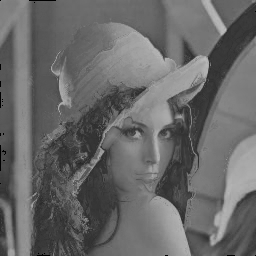
\includegraphics[scale=0.9]{itk-sym-lena.png}}
    \put(25,242){\begin{minipage}[t]{\linewidth}
    {Resultado obtido pela ITK}
    \end{minipage}}
  \end{picture}
\end{frame}

\begin{frame}
  \begin{picture}(320,250)
    \put(25,10){
\includegraphics[scale=0.9]{lenasymmetric.png}}
    \put(25,242){\begin{minipage}[t]{\linewidth}
    {Resultado obtido pelo demons simétrico.}
    \end{minipage}}
  \end{picture}
\end{frame}

\begin{frame}
  \begin{picture}(320,250)
    \put(25,10){
\includegraphics[scale=0.9]{lenaasymmetric.png}}
    \put(25,242){\begin{minipage}[t]{\linewidth}
    {Resultado obtido pelo demons asimétrico.}
    \end{minipage}}
  \end{picture}
\end{frame}

\begin{frame}
  \begin{picture}(320,250)
    \put(-5,140){
\includegraphics[scale=0.4]{lenaStatic.png}}
    \put(-5,130){\begin{minipage}[t]{0.4\linewidth}{Referência}\end{minipage}}
    \put(100,140){
\includegraphics[scale=0.4]{lenaMoving.png}}
    \put(100,130){\begin{minipage}[t]{0.4\linewidth}{Movel}\end{minipage}}
    \put(205,140){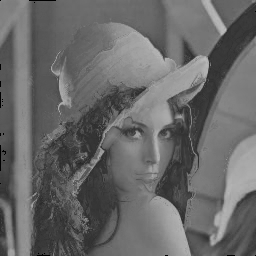
\includegraphics[scale=0.4]{itk-sym-lena.png}}
    \put(205,130){\begin{minipage}[t]{0.4\linewidth}{Resultado ITK}\end{minipage}}
    \put(35,20){
\includegraphics[scale=0.4]{lenasymmetric.png}}
    \put(35,10){\begin{minipage}[t]{0.4\linewidth}{Simétrico}\end{minipage}}
    \put(140,20){
\includegraphics[scale=0.4]{lenaasymmetric.png}}  
    \put(140,10){\begin{minipage}[t]{0.4\linewidth}{Asimétrico}\end{minipage}}
  \end{picture}
\end{frame}

\end{document}
